%% Atmospheric Environment (Elsevier) -- research paper
%% Compile: pdflatex -> bibtex -> pdflatex -> pdflatex
\documentclass[preprint,review,12pt,number,sort&compress]{elsarticle}

\usepackage[T1]{fontenc}
\usepackage{lmodern}
\usepackage[utf8]{inputenc}
\usepackage{graphicx}
\usepackage{amsmath,amssymb}
\usepackage{booktabs}
\usepackage{enumitem}
\usepackage{url}
\usepackage{lineno}
\usepackage{rotating}

\newcommand*{\ugm}{\ensuremath{\mu\mathrm{g\,m^{-3}}}}
\newcommand*{\pmten}{\ensuremath{\mathrm{PM_{10}}}}
\setlist[enumerate]{itemsep=2pt,topsep=4pt}
\emergencystretch=1.5em

\journal{Atmospheric Environment}

\begin{document}

\begin{frontmatter}

\title{A global reanalysis reproduces when, but not where, PM$_{10}$ is high across the dense
monitoring network of an arid emirate}

%% ORCIDs (enter in the submission system), as recorded for ATMENV-D-26-01869:
%% Jin Yoo 0000-0002-7738-8424; Jeongyun Kim 0009-0004-1377-8572;
%% Doo-Hee Lee 0000-0002-5116-2064; Ku Kang 0000-0001-8739-218X.
\author[cbrn]{Jin Yoo\fnref{eq}}
\author[snu]{Jeongyun Kim\fnref{eq}}
\author[kma]{Doo-Hee Lee}
\author[cbrn]{Ku Kang\corref{cor}}
\ead{bisu9082@gmail.com}

\cortext[cor]{Corresponding author.}
\fntext[eq]{These authors contributed equally to this work.}

\affiliation[cbrn]{organization={CBRN Defense Research Institute, Korea Ministry of National Defense},
  city={Seoul}, postcode={06796}, country={Republic of Korea}}
\affiliation[snu]{organization={Department of Chemical and Biological Engineering, Seoul National University},
  city={Seoul}, postcode={08826}, country={Republic of Korea}}
\affiliation[kma]{organization={Department of Civil Engineering and Environmental Sciences, Korea Military Academy},
  city={Seoul}, postcode={01805}, country={Republic of Korea}}

\begin{abstract}
Where monitors are few, exposure to coarse particulate matter (\pmten{}) is increasingly
assessed from global reanalyses, sometimes after statistical correction. We use the
regulatory network of the Emirate of Abu Dhabi (19 monitors, 16 of which share a $0.75^{\circ}$
cell of the CAMS reanalysis with another monitor) to measure what such a product represents. The
archived observations proved to be 24-h running means and were compared with the reanalysis
averaged over the same 24~h, October 2022 to May 2024 (32,566 three-hourly values; 5,989
monitor-days). The reanalysis reproduced when \pmten{} was high: the daily network-median level
correlated with its model counterpart at 0.67 (Spearman). It did not reproduce where. Mean bias
ranged from $-128$ to $+40$~\ugm{} and was spatially organised. Over the Abu Dhabi conurbation a
regional deficit that grew with the regional level in both seasons, shared by the inland city of
Al~Ain, was compounded by a local deficit of about 50--60~\ugm{} present on the cleanest
days. Of the
between-monitor variance of mean \pmten{}, 46\% lay inside single model cells (31\% for medians).
A gradient-boosted correction from the model value, date and position gave no established gain
at a monitor treated as unmonitored; an
apparent gain of 28--34\% arose only when running means were compared with instantaneous model
values. Mean \pmten{} exceeded the WHO 24-h guideline value at every monitor; the reanalysis had
little chance-corrected skill for exceedance (equitable threat score 0.09). Statements about
\pmten{} at a particular place require a measurement there.
\end{abstract}

\begin{highlights}
\item Archived PM$_{10}$ of the Abu Dhabi network are 24-h running means, not hourly values
\item CAMS tracked the regional daily level (Spearman 0.67) but not its spatial pattern
\item Up to half of the between-monitor PM$_{10}$ variance lay inside single model cells
\item The conurbation carried a local deficit of 50--60 \ugm{} even on the cleanest days
\item A correction from model value, date and position did not transfer to new sites
\end{highlights}

\begin{keyword}
PM$_{10}$ \sep CAMS reanalysis \sep Spatial representativeness \sep Sub-grid variability \sep
Running mean \sep Bias correction \sep Arabian Gulf
\end{keyword}

\end{frontmatter}

\linenumbers

\section{Introduction}

Coarse particulate matter is a persistent air-quality problem across the Arabian Gulf. Mineral
dust lifted from the surrounding deserts dominates the regional aerosol burden
\citep{gandham2020,shahid2026}, dust storms recur over the Emirates
\citep{barbulescu2020,karagulian2019}, and dust from Middle Eastern source areas reaches urban
receptors far downwind \citep{givehchi2013}. Local sources add to this regional background:
exhaust and non-exhaust traffic emissions, resuspended road dust, construction and industry
\citep{thorpe2008,amato2009,harrison2021}, which together make up the urban increment of
\pmten{} over its regional level \citep{lenschow2001}. The sources of \pmten{} have been
characterised for Kuwait \citep{hopke2026} and its variability described for Abu Dhabi
\citep{abuelgasim2020}, and the deposition of particle-bound species has been shown to vary
between sites with meteorology and surface geology \citep{bae2025be7}. The resulting exposure
matters for the burden of disease attributed to particulate matter
\citep{cohen2017,lelieveled2015,chen2020,orellano2020}, including during desert dust episodes
\citep{karanasiou2012}, yet routine surface monitoring is sparse across most of the Peninsula.
Where no monitor exists, assessments of exposure and of guideline exceedance fall back on models,
as hazard assessments in general do when measurements are unavailable \citep{shin2026resilient}:
for particulate matter, on global atmospheric-composition products such as the Copernicus
Atmosphere Monitoring Service (CAMS) reanalysis \citep{inness2019,flemming2015,morcrette2009},
MERRA-2 \citep{gelaro2017,randles2017}, or surface fields that fuse such models with satellite
retrievals \citep{van_donkelaar2016,hammer2020}.

Two properties of these products limit what they can say about \pmten{} at a point. The first is
skill at the surface. Aerosol data assimilation constrains the column optical depth, not the
surface mass concentration. The aerosol optical depth of these products has been validated
worldwide and over Arabia \citep{eskes2015,gueymard2020,labban2023}, but an evaluation against
surface particulate measurements in the Middle East found substantial differences \citep{ukhov2020}. The second is
representativeness. A grid value is an average over several thousand square kilometres and a
monitor samples one location inside that area, so the two would differ even if the model were
perfect \citep{schutgens2016,schutgens2017,janjic2018}; the area that a monitor represents
depends on the sources around it \citep{janssen2012,righini2014,duyzer2015}. For well-mixed,
long-lived constituents
the difference is small. For coarse particles in an arid city it need not be, because roads,
construction sites, industrial yards and bare soil are much smaller than a grid cell and the
particles they emit deposit within kilometres. The effect of sub-grid variability on exposure
estimates has been quantified for Europe \citep{denby2011,denby2024} and addressed by sub-grid
downscaling of regional models \citep{theobald2016}, but how large it is over the Gulf has rarely
been measured, because it takes several monitors inside one model cell to measure it. Representativeness also has a temporal side: a model value and an observation are comparable
only if they are averaged over the same interval \citep{schutgens2017}, and public archives do not
always state the interval over which a regulatory network reports.

The usual remedy for model error is statistical. A correction model is fitted to the difference
between observations and the gridded field at monitored locations and is then applied wherever
the field is available \citep{djalalova2015,huang2017}; for CAMS this has been done for
\pmten{} in dust forecasting \citep{sarafian2025} and for ozone at urban stations
\citep{kaffashzadeh2024}. Alternatively, point measurements are interpolated into continuous
fields, whose accuracy depends on the spatial structure of the field being mapped
\citep{kang2026mapping}. Whether such a correction
carries to places without monitors is normally judged by withholding one station at a time. In a
dense network that test is weaker than it looks, because the withheld station's neighbours remain
in the training set a few kilometres away, sampled on the same days and often inside the same
model cell \citep{roberts2017,ploton2020,meyer2021aoa,wadoux2021}, a problem for which
dedicated designs of spatial cross-validation have been proposed
\citep{valavi2019,mila2022,linnenbrink2024,meyer2022global}. The question is the
representativeness question seen from the other side: if what the gridded field misses is local,
a correction can only be learned from monitors that share that locality.

The regulatory network of the Emirate of Abu Dhabi allows these questions to be put to data.
Nineteen \pmten{} monitors lie at a median nearest-neighbour separation of 6.5~km, and sixteen of
them share a $0.75^{\circ}$ CAMS cell with at least one other monitor. We use this network to ask
(i) over what interval the archived values are averaged, and what follows for comparison with a
model; (ii) which part of the observed variability the CAMS reanalysis reproduces, separating the
day-to-day level of the region from the differences between places; (iii) how much of the spatial
variability lies inside single model cells, where a gridded product has one value to offer;
(iv) whether a statistical correction fitted at monitored sites improves the reanalysis at a site
treated as unmonitored; and (v) what the answers imply for assessing exceedance of the World
Health Organization 24-h guideline\footnote{World Health Organization, 2021. WHO global air quality guidelines: particulate matter (PM$_{2.5}$ and PM$_{10}$), ozone, nitrogen dioxide, sulfur dioxide and carbon monoxide. ISBN 978-92-4-003422-8. \url{https://www.who.int/publications/i/item/9789240034228}.}. A recent evaluation in this journal showed
that global reanalyses cannot reproduce the seasonal and diurnal cycles of surface ozone in a
data-sparse tropical region \citep{vieira2023}; the present study addresses the spatial
counterpart of that problem for coarse particles in an arid one.

\section{Data and methods}

\subsection{Surface observations}
\label{sec:obs}

\pmten{} from the 19 monitors operated by the Environment Agency -- Abu Dhabi was taken from the
OpenAQ open-data archive \citep{rosales2025} (Figure~\ref{fig:map}, Table~\ref{tab:stations}).
The archive holds 98,459 hourly \pmten{} values for these monitors between 29~October 2022 and
20~May 2024. Its coverage is uneven: from October 2022 to January 2023 it holds 14 of the 24
hours of the day, in February, May and July 2023 a single value per day at 08~UTC, in April and
June 2023 twelve hours, and from August 2023 onwards all hours; March 2023 is absent
(Supplementary Information, Section~S1). No value is negative and no upper cap was applied.

Two observation records are formed from the archive. The \emph{three-hourly record} holds the
archived value at every three-hourly time step of the reanalysis, 32,566 values, between 1,678
and 1,774 per monitor. The \emph{daily record} holds one value per monitor and day, the value at
08~UTC, which is the only hour the archive holds in every month: 5,989 monitor-days on 331 days.
The 20,818 three-hourly values up to December 2023 that were analysed in earlier work on this
network were checked against the archive and are identical to the archived values at the same
time stamps.

Each monitor carries the type assigned by the network operator and published by the Statistics
Centre -- Abu Dhabi\footnote{Statistics Centre -- Abu Dhabi, Air Quality Statistics: Methodology. \url{https://scad.gov.ae} (accessed 13 November 2026).}: industrial (four monitors), traffic (three), urban
(three), suburban (seven) and rural background (two). We use this classification as given and do
not reassign any station.

\subsection{The archived values are 24-h running means}
\label{sec:running}

The archived \pmten{} values are not hourly concentrations. Four properties of the record show
that each is an average over about 24~h (Section~S2). (i) Successive hourly values are almost
identical: the lag-1~h autocorrelation has a median of 0.996 across the monitors, all values are
integers, and 35\% of them equal the value one hour earlier. Nitrogen dioxide, sulfur dioxide,
ozone and carbon monoxide reported by the same stations in the same files have lag-1~h
autocorrelations of 0.80 to 0.91. (ii) For a trailing 24-h running mean $x$ of hourly
concentrations $h$, $x_t-x_{t-1}=(h_t-h_{t-24})/24$, so each hourly increment is undone 24~h
later and the increments are negatively correlated with themselves at that lag. The
autocorrelation of the hourly \pmten{} increments at 24~h is negative at all 19 monitors (median
$-0.36$, range $-0.53$ to $-0.19$); for the four gases the median is positive ($+0.06$ to
$+0.33$), as a diurnal cycle requires. (iii) The observed values correlate better with the mean
of the reanalysis over the preceding 24~h than with the reanalysis at the same instant (median
Pearson $r$ over the monitors 0.50 against 0.37), and in the three-hourly record to December 2023
the correlation falls at 17 of 19 monitors as the 24-h window is moved from trailing to centred
to leading. (iv) The national guideline for the Emirati Air Quality Index prescribes a 24-h
rolling average for \pmten{}, formed from at least 18 valid hourly values\footnote{Guideline for calculating the Emirati Air Quality Index (EAQI), 2023. \url{https://airquality.ncm.gov.ae/resources/pdf/aqi-quickguide-en-2023.pdf} (accessed 13 November 2026).}.

We therefore treat every archived value as the mean concentration over the 24~h ending at its
time stamp. Three consequences follow. The model counterpart of an archived value must be averaged
over the same 24~h (Section~\ref{sec:cams}). Values three hours apart share 21 of their 24 hours,
so that the daily record is used wherever independence in time matters. And the record contains
no information on the diurnal cycle or on peaks shorter than a day; the hourly concentrations
cannot be recovered from integer-rounded running means.

\subsection{Reanalysis and matched averaging}
\label{sec:cams}

Surface \pmten{} from the CAMS global reanalysis EAC4 \citep{inness2019}, whose aerosol scheme is
described by R\'emy et al.~\citep{remy2019}, was retrieved from the Copernicus Atmosphere Data Store at
$0.75^{\circ}$ and three-hourly resolution for 1~October 2022 to 31~May 2024 without gaps, and
converted to \ugm{}. Each monitor was matched to the nearest grid point. The 19 monitors occupy
nine cells; six cells hold two or more monitors and account for 16 of the 19
(Figure~\ref{fig:map}). Fifteen of the 171 monitor pairs share a cell, at separations from 1.0 to
46~km. The retrieved series reproduces, to within $2\times10^{-5}$~\ugm{}, all 20,818 model values
used in earlier work on this network.

For an archived value at time $t$ the model counterpart is the mean of the eight three-hourly
model values in the 24~h ending at $t$. Because the model series is continuous, every value of
both observation records has a counterpart. Comparing the archived values with the model at the
same instant instead, as an hourly record would be treated, changes the mean bias of a monitor by
at most 2~\ugm{}, but lowers the correlation in time and, as Section~\ref{sec:res-transfer}
shows, alters the verdict on statistical correction.

\subsection{Error structure, sub-grid variability and the regional level}

For each monitor we computed, on the three-hourly record, the mean bias (CAMS minus observed),
mean absolute error, root-mean-square error, and the Pearson and Spearman correlations between
the matched model and observed series. Spatial organisation of the mean bias was measured with
Moran's $I$ \citep{moran1950} in distance bands, with significance from 9,999 permutations of the station labels.

Sub-grid variability was measured in three ways. First, for each cell holding two or more
monitors we took the range and standard deviation of the monitors' mean observed concentrations,
and partitioned the between-monitor sum of squares of mean concentration over all 19 monitors
into a within-cell and a between-cell part; the partition was repeated on station medians, which
a single episode cannot dominate. Second, for every pair of monitors we computed the Spearman correlation \citep{spearman1904} of their observed three-hourly series over common time steps (at least 100) and
compared same-cell pairs with the correlation between each monitor and its own matched model
series. Third, for each pair we counted how often the two monitors lay on opposite sides of the
guideline value of 45~\ugm{}, over common time steps and over days of the daily record. A gridded
product that assigns the two monitors one value is necessarily wrong for one of them on every such
occasion.

To separate the timing of high concentrations from their location, each day of the daily record
with values from at least ten monitors was characterised by the median over the monitors (the
\emph{regional level}), for the observations and for the matched model values. Days were divided
into terciles of the observed regional level, and the bias and the spread between monitors were
computed within each tercile. The stability of the results over time was checked by repeating
the daily comparison for four sub-periods.

The association between station type and bias was tested with a Kruskal--Wallis test across the
five types \citep{kruskal1952} and, separately, with a one-sided Mann--Whitney test
\citep{mann1947} and a 200,000-draw permutation
test contrasting the monitors typed industrial, traffic or urban with those typed suburban or
rural background. The two-group contrast was formed after the five-group result was known; both
are reported.

\subsection{Statistical correction at a monitor treated as unmonitored}
\label{sec:methods-transfer}

The correction is a gradient-boosted regression \citep{friedman2001,pedregosa2011} of the
observed-minus-model difference on the matched model value, the sine and cosine of the hour and
of the day of the year, and latitude and longitude; a coordinate-free variant omits the last two.
Each monitor in turn is treated as unmonitored: the regression is trained on other monitors only
and its prediction, added to the model value, is compared with the withheld observations. The
gain is expressed as $\Delta=\log(\mathrm{MAE_{raw}}/\mathrm{MAE_{corrected}})$, so that
$\Delta>0$ means the correction reduced the mean absolute error. The three-hourly record is used,
after a screen that removes runs of six or more identical consecutive values (431 values, 1.3\%),
which leaves 32,135 values.

Withholding a monitor does not by itself make it unmonitored, because information about it
remains in the training data. Three kinds are removed in turn:
\begin{enumerate}
\item \emph{Nearby monitors.} All training monitors within a radius $R$ of the target are
      withheld, for $R=0$, 25, 50 and 100~km; $R=0$ is leave-one-station-out.
\item \emph{Observations from the same days.} The target record is cut into six blocks holding
      equal numbers of values, and each block is predicted from training data lying outside the
      block and outside a guard interval of ten days on either side. The matched residual stays
      correlated at this lag (median autocorrelation $+0.37$ at one day, $+0.18$ at three days
      and $+0.12$ at ten days), so no guard within the record makes the training data independent
      of the block; a three-day guard is reported as a check (Section~S5).
\item \emph{Monitors sharing the model cell.} Every training monitor in the target's CAMS cell
      is withheld, because it carries the same model series as the target.
\end{enumerate}
The test is an exact two-sided sign test on the 19 per-monitor values of $\Delta$, corrected by
the Benjamini--Hochberg procedure \citep{benjamini1995} across the 24 combinations of radius,
feature set and stage. Intervals for the median $\Delta$ are from 2,000 bootstrap resamples of
the nine occupied cells, the unit within which monitors share a model series \citep{efron1979}.
To show what the averaging interval does to this analysis, it was repeated on the same values
with the instantaneous model value in place of the matched one.

\subsection{Exceedance of the 24-h guideline}

Because the archived values are 24-h means, exceedance of the WHO 24-h guideline value can be
read from them directly. The daily record was used, with its matched model counterpart: 5,989
monitor-days. The observed value was classed as exceeding 45~\ugm{} or not and compared with the
same classification of the matched reanalysis. We report the probability of detection (POD), the
probability of false detection (POFD) and two scores that discount agreement expected by chance,
the equitable threat score (ETS) and the Heidke skill score (HSS); both are equitable only in
the limit of large samples \citep{hogan2010}. Intervals are from 2,000
bootstrap resamples of monitors. Two references that use the monitor itself indicate what local
information adds: the reanalysis shifted by the mean observed-minus-model difference at that
monitor over its preceding eight daily values, and persistence of the monitor's value from the
previous day. Neither is available where there is no monitor.

\section{Results}

\subsection{PM$_{10}$ exceeds the guideline at every monitor, and the reanalysis bias is organised
in space}
\label{sec:res-bias}

Mean observed \pmten{} ranges from 54 to 179~\ugm{} across the network
(Table~\ref{tab:stations}). Every one of the 19 station means lies above the 24-h guideline value
of 45~\ugm{}, and between 58\% and 99\% of the archived 24-h means at a monitor exceed it. Of the
5,989 monitor-days, 84\% exceed the guideline, from 60--68\% in the cleanest winter months to
more than 90\% from May to September 2023 (Section~S1), in line with the summer maximum reported
for the emirate in 2017--2018 \citep{abuelgasim2020}.

The matched reanalysis places the same locations between 37 and 106~\ugm{}. Its mean bias ranges
from $-128$~\ugm{} at Al~Mafraq to $+40$~\ugm{} at Sweihan, with a station mean of $-27$~\ugm{};
the median absolute error is 30~\ugm{} and the median root-mean-square error 48~\ugm{}. The model
does not reproduce which locations are high. Across the 19 monitors the standard deviation of
mean concentration is 27~\ugm{} in the observations and 19~\ugm{} in the model, and the two sets
of means are, if anything, inversely related (Spearman $\rho=-0.45$, $p=0.05$): the model's
highest values lie over the eastern desert, the observed ones in and around the city of Abu Dhabi.

The bias is not scattered at random. Moran's $I$ of the station mean bias is 0.80 for pairs
within 15~km ($p=0.001$) and 0.41 for pairs within 100~km ($p<0.001$). The seven monitors of the
Abu Dhabi metropolitan area are all underestimated, by 38 to 128~\ugm{}, whereas the four
monitors in Al~Ain, more than 100~km inland, are reproduced to within $-7$ to $+5$~\ugm{}
(Figure~\ref{fig:map}). The operator's station typology accounts for part of this pattern but not
cleanly. Monitors typed industrial, traffic or urban are underestimated by a median 55~\ugm{} and
suburban and rural-background monitors by a median 4~\ugm{} (Mann--Whitney $p=0.019$; permutation
$p=0.015$; Cohen's $d=-1.04$), but the five types taken separately do not differ significantly
(Kruskal--Wallis $p=0.23$), and each source-oriented type contains a monitor with little bias:
Ruwais (industrial, $-1$~\ugm{}), Al~Ain Street (traffic, $-7$~\ugm{}) and Zakher (urban,
$+5$~\ugm{}). Type alone does not predict where the reanalysis fails; location does. The pattern
is stable in time: the ranking of the monitors by daily mean bias in each of four sub-periods
agrees with that of the whole record (Spearman 0.92 to 0.98; Section~S4).

\subsection{Up to half of the spatial variance lies inside single model cells}
\label{sec:res-subgrid}

Table~\ref{tab:cells} and Figure~\ref{fig:subgrid}a show the six cells that hold more than one
monitor. In four of them the station means agree to within 1--16~\ugm{}. In the other two they do
not: station means differ by 56~\ugm{} in the cell containing E11~Road, Habshan South and Bida
Zayed, and by 89~\ugm{} in the cell containing Al~Mafraq, Mussafah and Baniyas, with within-cell
standard deviations of 30 and 46~\ugm{}. Over the whole network 46\% of the between-monitor
variance of mean \pmten{} lies within cells. The two high-spread cells differ in kind. The spread
in the E11~Road cell comes mainly from one episode between late August and mid-September 2023,
during which the 24-h mean at that roadside monitor reached 2,978~\ugm{}; its median (61~\ugm{})
is close to those of its neighbours, and on station medians the within-cell share of the variance
is 31\%. The spread in the Al~Mafraq cell, an industrial area south-east of Abu Dhabi island, is
persistent: the station medians there differ by more than 70~\ugm{}, and the range of station
means exceeds 100~\ugm{} in each sub-period of the daily record. In every sub-period between 42\%
and 51\% of the variance of station means, and between 35\% and 44\% of that of station medians,
lies within cells (Section~S4). No field on this grid, however accurate as a cell average, can
represent that part of the variability.

The six cells also separate two kinds of error that a single bias statistic merges. In the two
cells over Abu Dhabi island and its mainland suburbs the paired monitors agree closely (ranges of
1~\ugm{} each), yet the model lies 56 and 55~\ugm{} below them. There the discrepancy is not the
idiosyncrasy of one monitor; it is an urban-scale enhancement that the cell value does not carry.
In the two high-spread cells, by contrast, the monitor closest to the model is within 6 and
38~\ugm{} of it and the largest errors belong to individual industrial and roadside sites. In
Al~Ain the four monitors agree with each other and with the model.

For the guideline the consequence is direct. Two monitors in the same cell lie on opposite sides
of 45~\ugm{} in a median 10\% of common values, and in up to 39\% for the most dissimilar pair;
over days the figure is 14\% of 4,590 pair-days. A product with one value per cell is necessarily
wrong about exceedance at one of the two monitors on those days.

\subsection{The reanalysis reproduces when PM$_{10}$ is high, not where}
\label{sec:res-when}

In time the reanalysis does considerably better than in space. The observed regional level and
its model counterpart are related from day to day (Spearman $\rho=0.67$ over 327~days;
Figure~\ref{fig:regional}a), and the relation holds in each sub-period ($\rho=0.55$ to 0.71). At
single monitors the median Spearman correlation between the matched model and observed series is
0.55 (range 0.26 to 0.68; median Pearson $r=0.50$). This lies between the correlation of two
monitors that share a cell (median 0.66 over the 15 pairs) and that of monitors in different cells
(0.48; Figure~\ref{fig:subgrid}b): in time, the model stands in for a monitor somewhat better than
a distant monitor does, and somewhat worse than a neighbour. Proximity alone does not guarantee
coherence, however: the two monitors closest to each other, Khadeeja School and Hamdan Street,
1.0~km apart with mean concentrations of 95 and 93~\ugm{}, correlate at only 0.33.

What the reanalysis lacks is the difference between places, and that difference does not depend
on regional dust. When the days are divided by observed regional level, the Abu Dhabi
metropolitan monitors are underestimated by 46~\ugm{} in the lowest tercile (regional level 24 to
61~\ugm{}), by 58~\ugm{} in the middle one and by 86~\ugm{} in the highest (87 to 257~\ugm{}),
while the Al~Ain monitors move from $+13$ through 0 to $-23$~\ugm{}
(Figure~\ref{fig:regional}b). Two components are visible. A regional one, shared by the coast and
the interior, becomes more negative as the regional level rises: the model's day-to-day range is
compressed (regression slope of the model network median on the observed one 0.55), and its
network median exceeds 150~\ugm{} on 2 of the 327 days, against 12 in the observations. On top
of it, the conurbation carries an offset that does not change with the regional level: the
difference between the metropolitan and the Al~Ain bias is $-59$, $-57$ and $-63$~\ugm{} in the
three terciles. The spread between monitors behaves accordingly: the day-by-day standard
deviation across the network has a median of 27, 31 and 61~\ugm{} in the three terciles in the
observations, against 21, 22 and 25~\ugm{} in the model.

\subsection{A statistical correction gives no established gain, and the averaging interval
decides whether one appears}
\label{sec:res-transfer}

With each monitor withheld in turn and nothing else removed, the correction reduces the error at
13 of 19 monitors with coordinates as predictors (median $\Delta=+0.19$, cell-bootstrap interval
$+0.04$ to $+0.32$) and at 12 of 19 without them ($+0.11$, $-0.03$ to $+0.42$;
Figure~\ref{fig:transfer}a, Table~\ref{tab:transfer}). The sign test establishes neither
($p=0.17$ and 0.36 before correction for multiplicity). Withholding the monitors within 25~km
already brings the median to $+0.00$ for both feature sets. When the target record is predicted
in time blocks the gain disappears even with every neighbour retained (medians $+0.04$ and
$+0.02$, 11 and 10 of 19 monitors improved), and withholding the monitors of the target's cell
changes little further. None of the 24 comparisons differs from zero ($q=1.00$ for each). A
three-day guard gives the same result, with medians between $-0.28$ and $+0.09$ in the stages
with time blocks and no comparison different from zero (Section~S5).

The averaging interval is decisive for this conclusion. If the same 32,135 archived values are
compared with the model at the same instant, as an hourly record would be treated, the
leave-one-station-out gain is $+0.32$ with coordinates and $+0.42$ without, an apparent reduction
of the error by 28\% and 34\% at 17 and 16 of 19 monitors ($q=0.009$ and 0.015). This apparent
gain survives the controls that remove it under matched averaging: 16 of the 24 comparisons
establish it, including the coordinate-free correction with time blocks, the target's cell and
all monitors within 100~km withheld ($+0.15$, 15 of 19 monitors, $q=0.029$; Section~S5). In both
treatments the gain is carried by the day-of-year predictors; a correction given the model value
alone gains $+0.05$ under the instantaneous comparison and loses $-0.20$ under matched averaging
(Section~S5). What the correction learns from other monitors under the instantaneous comparison
is therefore mainly the mismatch in averaging, which all monitors share, and not something about
the atmosphere at the withheld site.

That no correction transfers under matched averaging is what Sections~\ref{sec:res-subgrid}
and~\ref{sec:res-when} predict. What the reanalysis misses at a monitor is largely a local offset;
other monitors do not carry that offset, and the regional signal that they do carry is already
in the model.

\subsection{Consequences for assessing guideline exceedance}
\label{sec:res-exceed}

Of the 5,989 monitor-days evaluated, 5,046 (84\%) exceed the guideline in the observations. With
a base rate this high a product that always reported exceedance would be right on five days in
six, and only scores that discount chance agreement are informative (Table~\ref{tab:exceed}).

The reanalysis detects 3,722 of the 5,046 exceedances (POD 0.74, 95\% interval 0.64 to 0.83) and
reports exceedance on 487 of the 943 days that did not exceed (POFD 0.52). Its equitable threat
score is 0.09 (0.03 to 0.15) and its Heidke skill score 0.16 (0.06 to 0.25): above chance, but
small. Shifting the reanalysis by the monitor's own recent mean difference, which adds knowledge
of the local level but none of the timing, raises the equitable threat score to 0.28 (0.24 to
0.32). Persistence of the monitor's previous day reaches 0.39 (0.34 to 0.44). The ordering is the
one the previous sections lead to. The reanalysis carries part of the day-to-day signal, but
whether a given place exceeds the guideline on a given day depends mostly on a local level that
the reanalysis does not contain and that only a monitor at the place supplies.

\section{Discussion}

\subsection{What the reanalysis error consists of}

The difference between a $0.75^{\circ}$ field and a point measurement contains model error and
representation error, and point data alone cannot fully separate them
\citep{schutgens2016,janjic2018}. The network nevertheless constrains the split in two ways.

First, the error is mostly an error of place. The reanalysis follows the day-to-day course of
the regional level, and at a single monitor it follows the observations better than a distant
monitor does. What it lacks is a set of offsets that differ from one location to the next, are
coherent over a few tens of kilometres, and vanish on average at the inland city of Al~Ain. Over
Abu Dhabi island and its suburbs four monitors in two cells agree with each other and jointly
exceed the model by more than 50~\ugm{}, so the discrepancy cannot be assigned to the siting of
one instrument.

Second, the error over the conurbation has two parts that respond differently to regional dust.
One is shared with the interior and grows with the regional level: the reanalysis compresses the
day-to-day range, overestimating the cleanest days at Al~Ain and underestimating the dustiest
days everywhere. This is the signature of an error in the amount of dust the model carries into
the region on high days. The other part is a difference between the
conurbation and the interior of about 60~\ugm{} that is the same on the cleanest days as on the
dustiest. An offset that does not respond to regional dust is not an error of dust transport. It
points instead to coarse particles of local origin, from traffic, construction, industry and resuspension \citep{thorpe2008,amato2009}, an urban
increment over the regional background \citep{lenschow2001} that a global model at this
resolution does not resolve, or to the composition of
the coastal cells, which extend over the sea as well as the city (Figure~\ref{fig:map}). The two
explanations are not exclusive, and this record cannot apportion the offset between them; that the
offset is constant argues against wind-driven resuspension as its main cause, because
resuspension would rise on the windy days that also bring regional dust.

Regulatory monitors are placed where exposure is expected to be high, so a network of this kind
overstates the deficit of a cell average and should not be read as an estimate of it. For the
question an assessment asks, namely what people at a given place breathe, the distinction matters
less than its size: between 31\% and 51\% of the spatial variance of \pmten{} in this
network is at scales the grid does not contain.

That the bias is spatially coherent but only loosely related to station type has a practical
corollary. A type-based adjustment, of the kind applied to make gridded products comparable with
urban or roadside monitors, would have been wrong here for at least one monitor in each
source-oriented class.

\subsection{The averaging interval of archived observations}

The values that an open archive holds for a regulatory network are whatever the network
publishes, and for particulate matter that may be the running mean on which an air-quality index
is based (Section~\ref{sec:running}), not the hourly concentration. In the present record the two are easy
to tell apart once the question is asked: hourly values that hardly change, increments that
reverse after 24~h, and gases from the same stations that behave otherwise. The same principle governs comparisons
between co-located instruments, where a systematic difference can arise entirely from what each
measured quantity includes \citep{you2026nai}. The check costs a
few lines of code and should precede any comparison of archived particulate data with a model.
The consequences of omitting it are not uniform. Mean bias and its spatial pattern were almost
unaffected here, because averaging does not change a mean. The correlation in time was
understated (0.37 instead of 0.50). And the evaluation of a statistical correction was
reversed: an apparent error reduction of 28--34\%, established at 16 and 17 of 19 monitors and
robust to every control applied, disappeared when model and observations were averaged alike.

\subsection{Why correction does not help, and what leave-one-station-out measures}

Statistical correction of chemical-transport output is well established where the corrected
product is used at the monitors that trained it \citep{djalalova2015,huang2017}, and the present
results are consistent with that use: knowledge of a monitor's own recent level raised the
exceedance score from 0.09 to 0.28. They do not support the further and common inference that a
correction fitted to a network can be mapped over areas without monitors. In this network the
leave-one-station-out gain was not established even before anything else was withheld (13 of 19
monitors improved), and it vanished once neighbours within 25~km were withheld or the training data
were separated from the target in time.
The requirement that a validation withhold what deployment will lack is familiar from
spatial prediction \citep{roberts2017,ploton2020,wadoux2021}, and the transferability of
statistical models between arid regimes has recently been examined for dust-related fine
particles \citep{hurynovich2026}. What the atmospheric setting adds is a physical reason for the
outcome. A correction can transfer only the part of the error that monitors share, and here the
shared part is the regional signal that the reanalysis already reproduces. The part that the
reanalysis misses is local, and no monitor elsewhere holds it. The conclusion applies to
corrections built, as this one is, from the model value, the date and the position; predictors
that describe the locality itself, such as land use, road density or emission inventories
\citep{zhang2018lur}, address the missing part directly and were not tested.

\subsection{Implications for assessment in arid, sparsely monitored regions}

Three implications follow for the use of reanalysis \pmten{} where monitors are few. First, a
reanalysis of this kind can indicate on which days \pmten{} over a region is high. It should not
be used to decide whether a particular place exceeded a guideline, and exceedance statistics
derived from it in a region where the guideline is exceeded on most days should be reported with
a chance-corrected score and the base rate. Second, the uncertainty attached to a grid value
used as a point estimate should include the sub-grid spread \citep{denby2011}, which in this network is as large
as the guideline value itself in the cells that contain strong local sources. Third, because the
missing component is a local level that changes slowly, a monitor informs its own site far more
than it informs a statistical model of the region; for a fixed number of instruments, coverage
of distinct source environments is worth more to assessment than replication within one.

\subsection{Limitations}
\label{sec:limits}

The study rests on one network in one emirate and on 19 months of record. The archive is thin in
spring and summer 2023, when it holds one value per day in three months, so the dust season is
represented mainly through the daily record. The archived values are integer-rounded 24-h running
means, so the study says nothing about diurnal variation or short peaks, and the alignment of the
averaging window, inferred from the data and from the national reporting convention, could not be
confirmed from station metadata. Point monitors sited for regulatory purposes are not a random
sample of a cell. A single global product at $0.75^{\circ}$ was evaluated; a regional simulation at
kilometre scale with resolved local emissions would be the proper test of how much of the
sub-grid variance is recoverable by resolution \citep{ukhov2020}. The correction analysis has 19
units and one model family. The contrast between source-oriented and background station types was
formed after an omnibus test had failed and is reported as such. Finally, the exceedance analysis
classifies 24-h means in retrospect; it is not a verification of forecasts.

\section{Conclusions}

The \pmten{} values that the open archive holds for the 19 regulatory monitors of the Emirate of
Abu Dhabi are 24-h running means, and they exceed the WHO 24-h guideline value on most days at
every monitor. Compared over the same averaging interval and over 19 months, the CAMS reanalysis
followed the day-to-day course of the regional level (Spearman 0.67) and tracked single monitors
better than a distant monitor did, but it did not reproduce the differences between places: the
mean bias ranged from $-128$ to $+40$~\ugm{} and was organised in space. Over the Abu Dhabi
conurbation it combined a regional deficit that grew on dusty days with a local offset of about
60~\ugm{} that did not change with the regional level, while the inland city of Al~Ain was
reproduced on average. Between 31\% and 51\% of the between-monitor variance of \pmten{} lay
inside single $0.75^{\circ}$ cells. A statistical correction trained on other monitors gave
no established gain at a monitor treated as unmonitored; the gain that appears when running means
are compared with instantaneous model values is produced by the mismatch in averaging. Judged by a chance-corrected score, the
reanalysis had little skill in separating days that exceeded the guideline at a monitor from days
that did not. In arid regions with strong local sources of coarse particles, a global reanalysis
describes when the regional background is high; statements about a particular place still require
a measurement there.


\section*{CRediT authorship contribution statement}
\textbf{Jin Yoo:} Conceptualization, Methodology, Software, Formal analysis, Writing -- original
draft. \textbf{Jeongyun Kim:} Data curation, Investigation, Writing -- review and editing.
\textbf{Doo-Hee Lee:} Methodology, Software, Formal analysis, Validation, Writing -- original
draft. \textbf{Ku Kang:} Conceptualization, Supervision, Writing -- review
and editing. Jin Yoo and Jeongyun Kim contributed equally to this work.

\section*{Declaration of competing interest}
The authors declare that they have no known competing financial interests or personal
relationships that could have appeared to influence the work reported in this paper.

\section*{Declaration of generative AI and AI-assisted technologies in the writing process}
During the preparation of this work the authors used Claude (Anthropic) to assist with drafting
and language editing of the manuscript text and with writing and debugging the analysis and
figure-generation code. All measurements and model fields were obtained from the cited public
archives; no data, numerical results or references were generated by AI. After using this tool
the authors reviewed and edited the content as needed, verified every reported numerical value
against the underlying artefacts, and take full responsibility for the content of the published
article.

\section*{Acknowledgements}
We thank the Environment Agency -- Abu Dhabi, the OpenAQ initiative and the Copernicus Atmosphere
Monitoring Service for open access to the data used in this study, and the AERONET project and
the principal investigator of the DEWA Research Centre site, Luis Mart\'in Pomares, and his staff
for establishing and maintaining the site whose data are used here, and the Iowa Environmental
Mesonet for the archive of airport weather reports.

\section*{Funding}
This research did not receive any specific grant from funding agencies in the public, commercial,
or not-for-profit sectors.

\section*{Data and code availability}
\sloppy
The hourly archive of the 19 monitors as retrieved from the OpenAQ public archive, the script
that retrieves it, the analysed three-hourly observation--model records, the analysis and figure
scripts and all result artefacts are available in the public repository
\url{https://github.com/bisu9082/camscast} under the MIT licence. The evidence on the
averaging interval is produced by \texttt{archive\_checks.py} and
\texttt{averaging\_fingerprint.py}, the station-level, sub-grid and regional statistics by
\texttt{station\_representativeness.py}, \texttt{extended\_observations.py} and
\texttt{revision\_diagnostics.py}, the sun-photometer comparison by
\texttt{fetch\_aeronet.py} and \texttt{aeronet\_dust\_check.py}, the airport reports by
\texttt{fetch\_metar\_omaa.py} and \texttt{metar\_dust\_check.py}, the dust and wind analysis by
\texttt{fetch\_cams\_eac4\_aod\_wind.py} and \texttt{dust\_wind\_analysis.py}, the exceedance
scores by \texttt{exceedance\_detection.py}, the tables by \texttt{make\_tables\_ae.py} and
Figures~\ref{fig:map}--\ref{fig:regional} by \texttt{make\_figs\_ae.py}. The raw CAMS EAC4 fields
are distributed by the Copernicus Atmosphere Data Store and are not redistributed; the request
parameters are documented in \texttt{data\_retrieval/RETRIEVAL.md}.

\bibliographystyle{elsarticle-num}
\bibliography{references}

\clearpage

\begin{table}[p]\centering\footnotesize
\caption{The 19 monitors: operator station type (Statistics Centre -- Abu Dhabi), coordinates, number of
values in the three-hourly record $N$ (29~October 2022 to 20~May 2024), mean observed \pmten{},
mean of the matched CAMS values (the mean over the 24~h ending at each observation), mean bias
(CAMS minus observed) and Pearson correlation $r$ between the matched model and observed series.
Concentrations in \ugm{}. Observed values are 24-h running means. Monitors are ordered by type
and, within type, by bias.}
\label{tab:stations}
\resizebox{\textwidth}{!}{\begin{tabular}{llrrrrrrr}\toprule
Monitor & Type & Lat & Lon & $N$ & Observed & CAMS & Bias & $r$ \\ \midrule
Al Mafraq & Industrial & 24.29 & 54.59 & 1{,}708 & 178.6 & 51.0 & $-127.6$ & 0.57 \\
Mussafah & Industrial & 24.35 & 54.50 & 1{,}705 & 115.2 & 51.2 & $-64.0$ & 0.25 \\
Habshan S. & Industrial & 23.75 & 53.75 & 1{,}710 & 64.7 & 47.7 & $-17.0$ & 0.48 \\
Ruwais & Industrial & 24.09 & 52.75 & 1{,}772 & 58.4 & 57.6 & $-0.8$ & 0.40 \\
E11 Road & Traffic & 24.04 & 53.89 & 1{,}678 & 110.0 & 47.7 & $-62.4$ & 0.41 \\
Hamdan St. & Traffic & 24.49 & 54.36 & 1{,}685 & 93.4 & 37.5 & $-55.9$ & 0.20 \\
Al Ain St. & Traffic & 24.23 & 55.77 & 1{,}685 & 86.2 & 79.3 & $-6.9$ & 0.65 \\
Khadeeja School & Urban & 24.48 & 54.37 & 1{,}733 & 94.5 & 38.1 & $-56.4$ & 0.44 \\
Al Maqtaa & Urban & 24.40 & 54.52 & 1{,}699 & 100.0 & 45.7 & $-54.3$ & 0.43 \\
Zakher & Urban & 24.16 & 55.70 & 1{,}759 & 74.6 & 79.6 & $+5.0$ & 0.58 \\
Khalifa City & Suburban & 24.42 & 54.58 & 1{,}696 & 101.1 & 45.7 & $-55.4$ & 0.51 \\
Baniyas School & Suburban & 24.32 & 54.64 & 1{,}733 & 89.2 & 51.1 & $-38.1$ & 0.70 \\
Gayathi & Suburban & 23.84 & 52.81 & 1{,}774 & 74.3 & 57.8 & $-16.5$ & 0.65 \\
Bida Zayed & Suburban & 23.65 & 53.70 & 1{,}688 & 53.9 & 47.9 & $-5.9$ & 0.51 \\
Al Tawia & Suburban & 24.26 & 55.70 & 1{,}711 & 82.8 & 79.5 & $-3.3$ & 0.72 \\
Al Ain Islamic & Suburban & 24.22 & 55.73 & 1{,}712 & 78.7 & 79.6 & $+0.9$ & 0.50 \\
Sweihan & Suburban & 24.47 & 55.34 & 1{,}695 & 66.2 & 106.2 & $+40.0$ & 0.68 \\
Al Qua'a & Rural background & 23.53 & 55.49 & 1{,}723 & 88.2 & 84.2 & $-4.0$ & 0.44 \\
Liwa & Rural background & 23.10 & 53.61 & 1{,}700 & 73.0 & 82.7 & $+9.7$ & 0.35 \\
\bottomrule\end{tabular}
}
\end{table}

\begin{table}[p]\centering\footnotesize
\caption{Sub-grid variability. For each $0.75^{\circ}$ CAMS cell holding two or more monitors:
the mean observed \pmten{} over the cell's monitors, the mean matched CAMS value, the offset
between them (CAMS minus observed), and the range and
standard deviation of the monitors' mean observed concentrations (all in \ugm{}). Monitors in a
cell receive the same model series.}
\label{tab:cells}
\resizebox{\textwidth}{!}{\begin{tabular}{ccclrrrrr}\toprule
\multicolumn{2}{c}{Cell centre} & & & \multicolumn{3}{c}{Mean PM$_{10}$} & \multicolumn{2}{c}{Between monitors} \\ \cmidrule(lr){1-2}\cmidrule(lr){5-7}\cmidrule(lr){8-9}
Lat & Lon & $n$ & Monitors & Observed & CAMS & Offset & Range & SD \\ \midrule
24.00 & 52.50 & 2 & Gayathi, Ruwais & 66 & 58 & $-9$ & 16 & 11.3 \\
24.00 & 54.00 & 3 & Bida Zayed, Habshan S., E11 Road & 76 & 48 & $-28$ & 56 & 29.8 \\
24.75 & 54.00 & 2 & Khadeeja School, Hamdan St. & 94 & 38 & $-56$ & 1 & 0.8 \\
24.00 & 54.75 & 3 & Mussafah, Baniyas School, Al Mafraq & 128 & 51 & $-77$ & 89 & 46.0 \\
24.75 & 54.75 & 2 & Khalifa City, Al Maqtaa & 101 & 46 & $-55$ & 1 & 0.8 \\
24.00 & 55.50 & 4 & Al Ain St., Al Ain Islamic, Zakher, Al Tawia & 81 & 79 & $-1$ & 12 & 5.0 \\
\bottomrule\end{tabular}
}
\end{table}

\begin{sidewaystable}[p]\centering\footnotesize
\caption{Gain of the statistical correction at a monitor treated as unmonitored, with model and
observations averaged over the same 24~h.
$\Delta=\log(\mathrm{MAE_{raw}}/\mathrm{MAE_{corrected}})$; the median is over the 19 monitors and
the interval is from 2,000 bootstrap resamples of the nine occupied model cells. ``Sources'' is
the mean number of training monitors remaining. ``Improved'' counts monitors with $\Delta>0$.
$q$ is the Benjamini--Hochberg-corrected exact two-sided sign test across the 24 comparisons.
Model and observations cover 29~October 2022 to 20~May 2024 (32,135 values after the flat-line
screen).}
\label{tab:transfer}
\resizebox{\textheight}{!}{\begin{tabular}{rrcrrcrr}\toprule
& & \multicolumn{3}{c}{With coordinates} & \multicolumn{3}{c}{Coordinate-free} \\ \cmidrule(lr){3-5}\cmidrule(lr){6-8}
$R$ (km) & Sources & Median $\Delta$ [95\% CI] & Improved & $q$ & Median $\Delta$ [95\% CI] & Improved & $q$ \\ \midrule
\multicolumn{8}{l}{\emph{Monitors within $R$ withheld}} \\
0 & 18.0 & $+0.186$ [$+0.040$, $+0.318$] & 13/19 & 1.000 & $+0.113$ [$-0.026$, $+0.422$] & 12/19 & 1.000 \\
25 & 15.5 & $+0.001$ [$-0.247$, $+0.163$] & 10/19 & 1.000 & $-0.000$ [$-0.189$, $+0.294$] & 9/19 & 1.000 \\
50 & 14.4 & $-0.158$ [$-0.492$, $+0.110$] & 7/19 & 1.000 & $-0.026$ [$-0.252$, $+0.294$] & 9/19 & 1.000 \\
100 & 12.0 & $-0.000$ [$-1.699$, $+0.324$] & 9/19 & 1.000 & $-0.191$ [$-0.368$, $+0.272$] & 9/19 & 1.000 \\
\multicolumn{8}{l}{\emph{+ time blocks with ten-day guard}} \\
0 & 18.0 & $+0.038$ [$-0.083$, $+0.243$] & 11/19 & 1.000 & $+0.016$ [$-0.280$, $+0.278$] & 10/19 & 1.000 \\
25 & 15.5 & $-0.111$ [$-0.352$, $+0.158$] & 8/19 & 1.000 & $+0.016$ [$-0.280$, $+0.197$] & 10/19 & 1.000 \\
50 & 14.4 & $-0.291$ [$-0.469$, $+0.091$] & 7/19 & 1.000 & $+0.008$ [$-0.264$, $+0.176$] & 10/19 & 1.000 \\
100 & 12.0 & $-0.000$ [$-1.584$, $+0.144$] & 9/19 & 1.000 & $-0.050$ [$-0.316$, $+0.183$] & 9/19 & 1.000 \\
\multicolumn{8}{l}{\emph{+ monitors sharing the model cell withheld}} \\
0 & 16.4 & $+0.091$ [$-0.140$, $+0.295$] & 11/19 & 1.000 & $+0.008$ [$-0.255$, $+0.287$] & 10/19 & 1.000 \\
25 & 15.2 & $-0.111$ [$-0.352$, $+0.165$] & 9/19 & 1.000 & $+0.008$ [$-0.255$, $+0.175$] & 10/19 & 1.000 \\
50 & 14.4 & $-0.291$ [$-0.469$, $+0.091$] & 7/19 & 1.000 & $+0.008$ [$-0.264$, $+0.175$] & 10/19 & 1.000 \\
100 & 12.0 & $-0.000$ [$-1.584$, $+0.144$] & 9/19 & 1.000 & $-0.050$ [$-0.316$, $+0.184$] & 9/19 & 1.000 \\
\bottomrule\end{tabular}
}
\end{sidewaystable}

\begin{table}[p]\centering\footnotesize
\caption{Exceedance of the WHO 24-h \pmten{} guideline value (45~\ugm{}) by monitor and day (24-h
mean ending 08~UTC), 29~October 2022 to 16~May 2024. POD: probability of detection; POFD: probability of
false detection; ETS: equitable threat score; HSS: Heidke skill score. Intervals are from 2,000
bootstrap resamples of monitors. The level-shifted reanalysis and persistence use the monitor's
own preceding values and are evaluated on the days for which those exist.}
\label{tab:exceed}
\resizebox{\textwidth}{!}{\begin{tabular}{llrrcccc}\toprule
Classifier & Local information & Days & Exceeding & POD [95\% CI] & POFD & ETS [95\% CI] & HSS [95\% CI] \\ \midrule
CAMS reanalysis & none & 5{,}989 & 5{,}046 & 0.738 [0.644, 0.829] & 0.516 & $0.088$ [$0.033$, $0.145$] & $0.163$ [$0.063$, $0.254$] \\
CAMS, level-shifted & own monitor, preceding 8 days & 5{,}073 & 4{,}253 & 0.920 [0.896, 0.942] & 0.495 & $0.281$ [$0.241$, $0.317$] & $0.439$ [$0.388$, $0.481$] \\
Persistence & own monitor, previous day & 4{,}761 & 4{,}021 & 0.934 [0.916, 0.950] & 0.372 & $0.395$ [$0.344$, $0.439$] & $0.566$ [$0.512$, $0.610$] \\
\bottomrule\end{tabular}
}
\end{table}

\begin{figure}[p]\centering
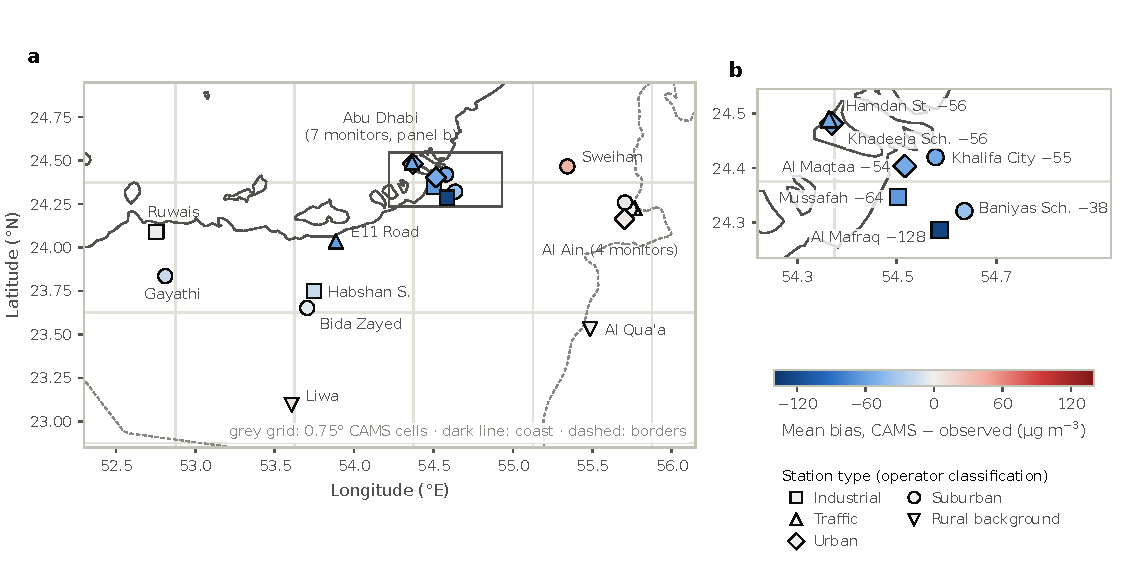
\includegraphics[width=\textwidth]{Fig1_map.pdf}
\caption{The Abu Dhabi regulatory \pmten{} network and the mean bias of the CAMS reanalysis.
(a) All 19 monitors; (b) the seven monitors of the Abu Dhabi metropolitan area, with mean bias in
\ugm{}. Colour gives the mean bias (CAMS minus observed) over each monitor's matched record and
marker shape the operator's station type. Grey lines are the boundaries of the $0.75^{\circ}$
model cells; the coastline and national borders are from Natural Earth.}
\label{fig:map}
\end{figure}

\begin{figure}[p]\centering
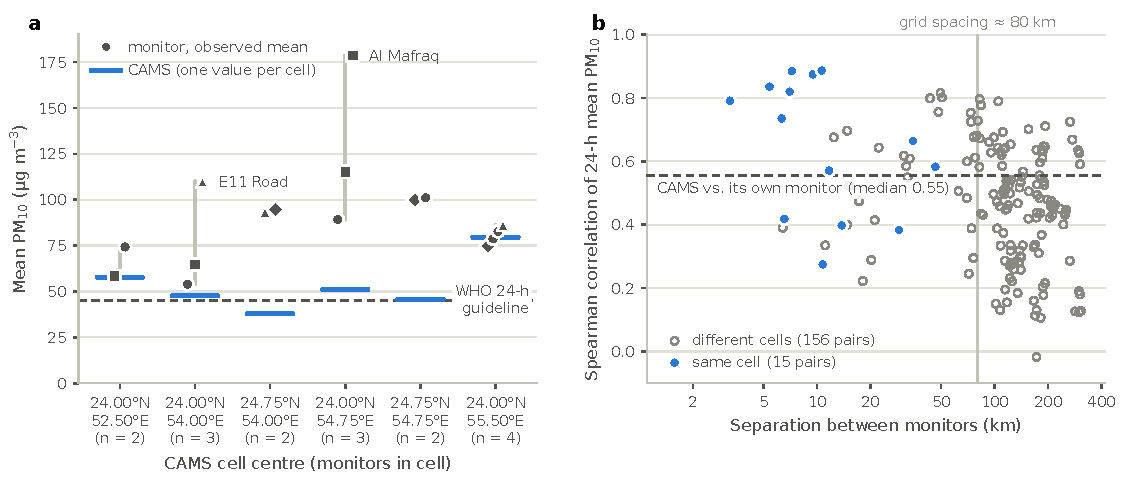
\includegraphics[width=\textwidth]{Fig2_subgrid.pdf}
\caption{Variability of \pmten{} below the scale of the model grid. (a) Mean observed \pmten{} at
each monitor in the six cells that hold more than one monitor (marker shape: station type, as in
Figure~\ref{fig:map}; grey bar: range within the cell), against the mean of the single model
series the cell supplies (blue) and the WHO 24-h guideline value (dashed). (b) Spearman
correlation between the observed series of each pair of monitors against their separation, for
pairs in the same model cell (filled) and in different cells (open); the dashed line is the
median correlation between a monitor and its own matched model series.}
\label{fig:subgrid}
\end{figure}

\begin{figure}[p]\centering
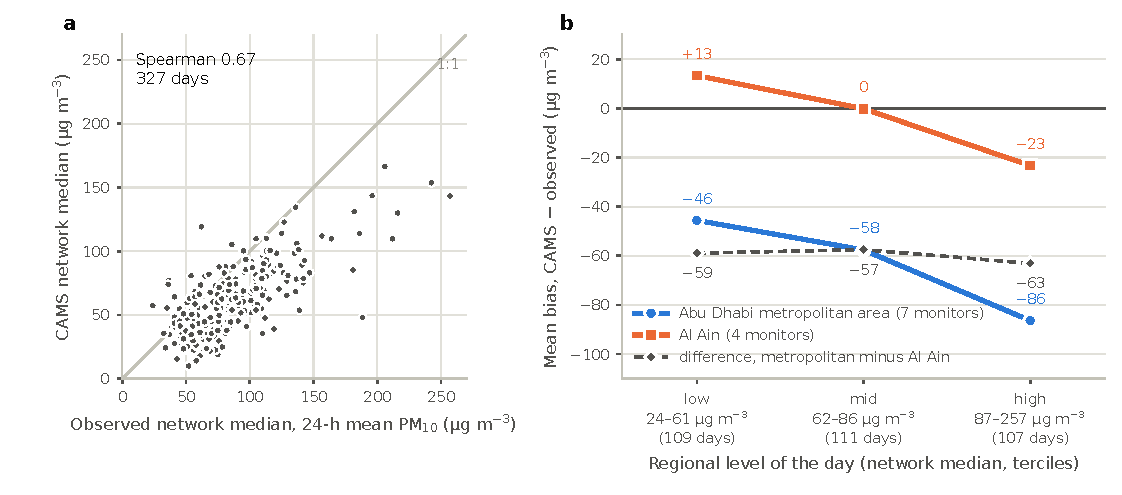
\includegraphics[width=\textwidth]{Fig3_regional.pdf}
\caption{What the reanalysis reproduces and what it does not. (a) Daily regional level (median
over the monitors of the 24-h mean ending 08~UTC) in the observations and in the matched
reanalysis, 327 days from October 2022 to May 2024. (b) Mean bias of the reanalysis at the
monitors of the Abu Dhabi metropolitan area and of Al~Ain, and the difference between the two
(dashed), for days divided into terciles of the observed regional level.}
\label{fig:regional}
\end{figure}

\begin{figure}[p]\centering
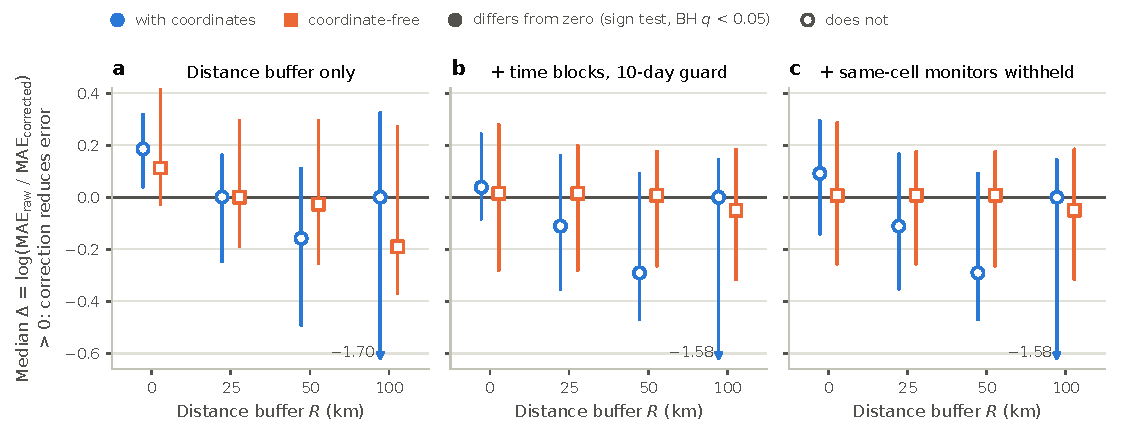
\includegraphics[width=\textwidth]{Fig4_transfer.pdf}
\caption{Gain of the statistical correction at a monitor treated as unmonitored, with model and
observations averaged over the same 24~h. Median $\Delta$ over the 19 monitors, with 95\%
intervals from a bootstrap over model cells, against the radius within which training monitors
are withheld. (a) Distance buffer only; $R=0$ is leave-one-station-out. (b) With the target
record additionally predicted in time blocks separated from training data by a ten-day guard.
(c) With monitors sharing the target's model cell also withheld. Filled markers differ from zero
by the sign test after Benjamini--Hochberg correction ($q<0.05$); open markers do not.
Intervals that extend below the plotted range are labelled with their lower limit.}
\label{fig:transfer}
\end{figure}

\end{document}
